\documentclass[tikz,border=10pt]{standalone}

\usepackage[latin1]{inputenc}
\usepackage{tikz}

% GNUPLOT required
\begin{document}
\pagestyle{empty}


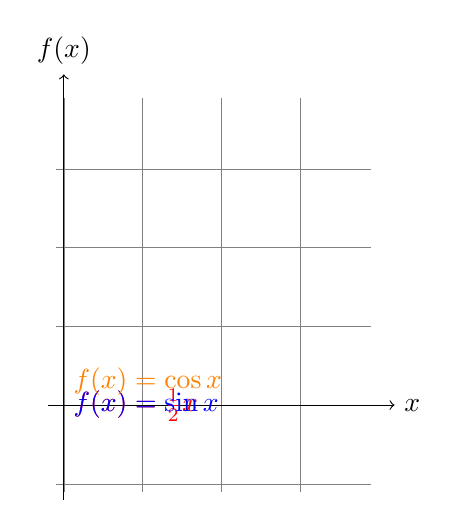
\begin{tikzpicture}[domain=0:4]
    \draw[very thin,color=gray] (-0.1,-1.1) grid (3.9,3.9);
    \draw[->] (-0.2,0) -- (4.2,0) node[right] {$x$};
    \draw[->] (0,-1.2) -- (0,4.2) node[above] {$f(x)$};
    \draw[color=red] plot[id=x] function{0.5*x}
        node[right] {$f(x) =\frac{1}{2}x$};
    \draw[color=blue] plot[id=sin] function{sin(x)}
        node[right] {$f(x) = \sin x$};
    \draw[color=orange] plot[id=cos] function{cos(x)}
        node[above right] {$f(x) = \cos x$};
\end{tikzpicture}


\end{document}
